\documentclass[a4paper,12pt]{article}
\usepackage[utf8]{inputenc}
\usepackage[ngerman]{babel}
\usepackage{geometry}
\usepackage{graphicx}
\usepackage{hyperref}

\title{Lebenslauf}
\author{Peter Kuhn}
\date{}

\begin{document}

\maketitle

\begin{minipage}{0.7\textwidth}
\section*{Personalien}
\begin{tabular}{ll}
Name: & Peter Kuhn \\
Adresse: & Webergasse 16, 8640 Rapperswil \\
Mobil: & 078 707 12 46 \\
Festnetz: & 043 268 55 87 \\
Geburtsdatum: & 1998-06-17\\
E-Mail: & \href{mailto:peterkuhn@peterkuhn.ch}{peterkuhn@peterkuhn.ch} \\
\end{tabular}
\end{minipage}
\hfill
\begin{minipage}{0.25\textwidth}
    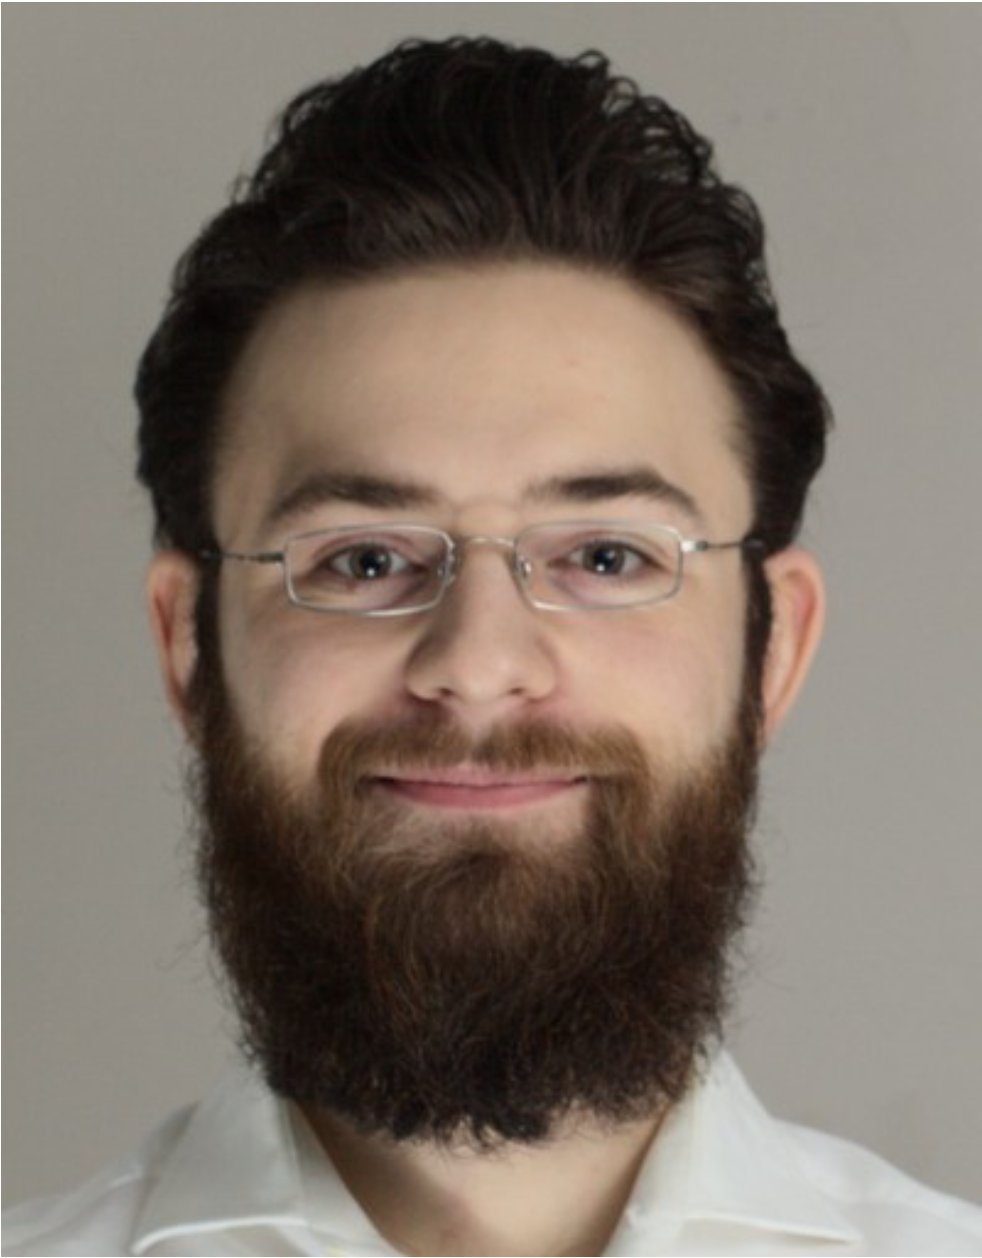
\includegraphics[width=\textwidth]{Portait}
\end{minipage}

\section*{Bildung}

2021 - jetzt Maschinenentechnik und Innovation Studium an der OST\\
2018 - 2020 Mathematik Studium ETH Zürich\\
2017 - 2018 Zivildienst\\
2013 - 2017 Kurzzeit Gymnasium Math. Naturwiss. Gym. Rämibühl\\
2011 - 2013 Langzeit Gymnasium Kantonsschule Zürcher Oberland\\



\href{http://peterkuhn.ch/Maturarbeit20170120.pdf}{Maturarbeit}

\section*{Sprachen}
\begin{itemize}
    \item Deutsch (Muttersprache)
    \item Englisch (sehr gut schriftlich und mündlich)
    \item Italienisch (gut mündlich)
\end{itemize}

\section*{Programmiersprachen}
Python (gut), Matlab (sehr gut), PostgreSQL (gut), C++ (basic), C (basic), Bash (basic), Java (basic)

\section*{Fähigkeiten}
\begin{itemize}
\item Führerausweis Kat. B
\item manuell Drehen und Fräsen

\end{itemize}

\section*{Sport}
\begin{itemize}
    \item Mountainbike
    \item Rennvelo
\end{itemize}

\end{document}
